\documentclass{standalone}
\usepackage{tikz}
\usetikzlibrary{patterns, positioning}


\begin{document}
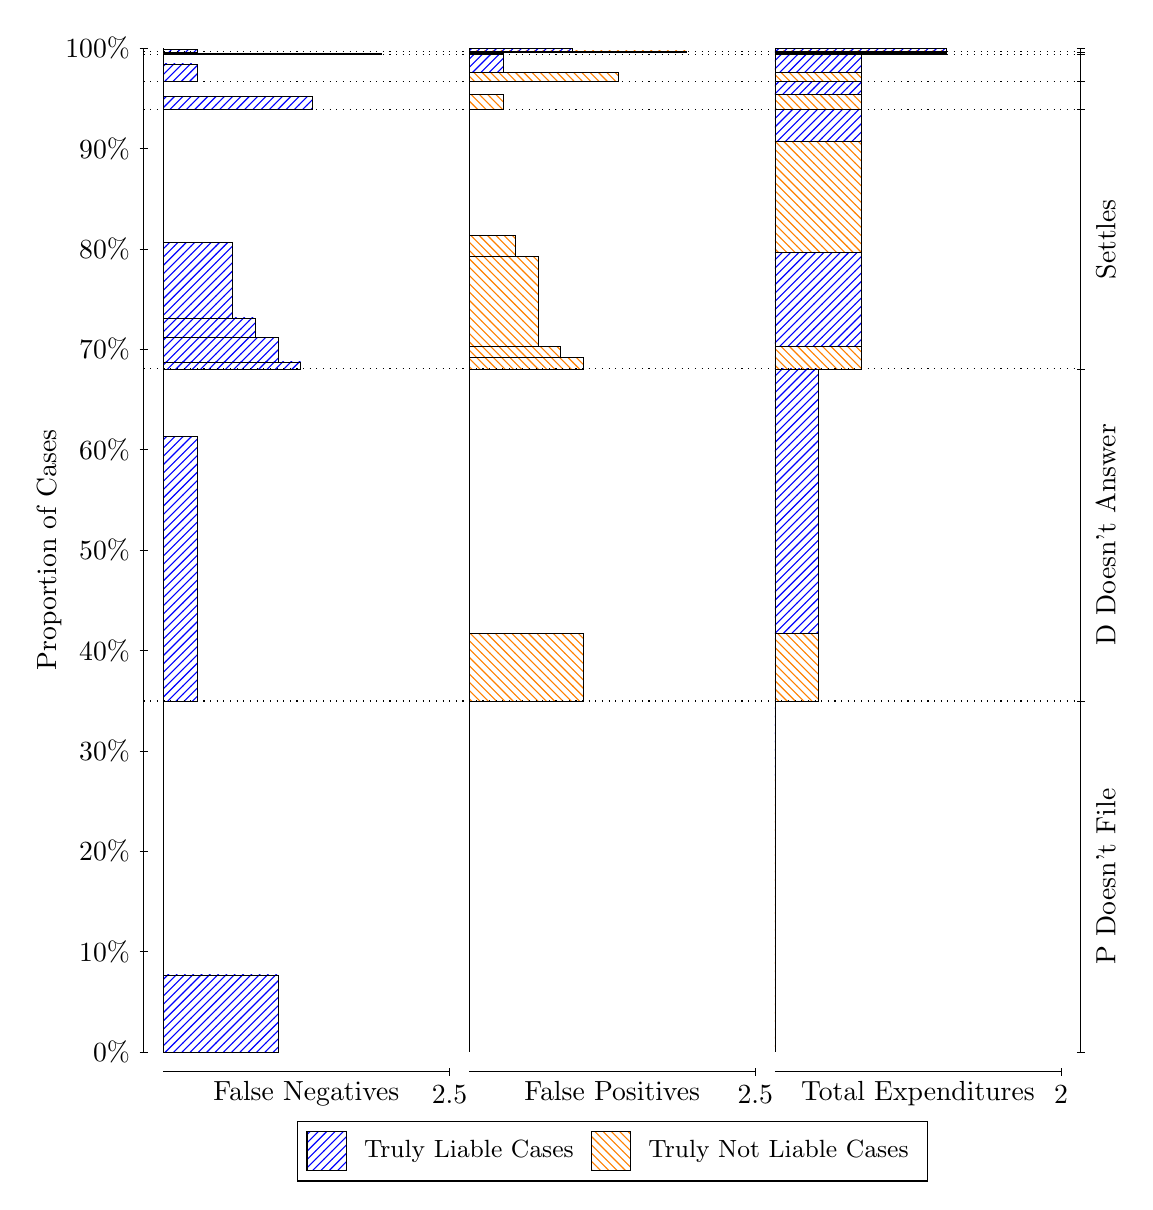
\begin{tikzpicture}
\draw[black, very thin] (1.5,1.75) -- (1.5,14.5);
\node[rotate=90, text=black, anchor=center] at (0.3, 8.125) {Proportion of Cases};
\draw[black, very thin] (1.45,1.75) -- (1.55,1.75);
\node[text=black, anchor=east] at (1.45, 1.75) {0\%};
\draw[black, very thin] (1.45,3.025) -- (1.55,3.025);
\node[text=black, anchor=east] at (1.45, 3.025) {10\%};
\draw[black, very thin] (1.45,4.3) -- (1.55,4.3);
\node[text=black, anchor=east] at (1.45, 4.3) {20\%};
\draw[black, very thin] (1.45,5.575) -- (1.55,5.575);
\node[text=black, anchor=east] at (1.45, 5.575) {30\%};
\draw[black, very thin] (1.45,6.85) -- (1.55,6.85);
\node[text=black, anchor=east] at (1.45, 6.85) {40\%};
\draw[black, very thin] (1.45,8.125) -- (1.55,8.125);
\node[text=black, anchor=east] at (1.45, 8.125) {50\%};
\draw[black, very thin] (1.45,9.4) -- (1.55,9.4);
\node[text=black, anchor=east] at (1.45, 9.4) {60\%};
\draw[black, very thin] (1.45,10.675) -- (1.55,10.675);
\node[text=black, anchor=east] at (1.45, 10.675) {70\%};
\draw[black, very thin] (1.45,11.95) -- (1.55,11.95);
\node[text=black, anchor=east] at (1.45, 11.95) {80\%};
\draw[black, very thin] (1.45,13.225) -- (1.55,13.225);
\node[text=black, anchor=east] at (1.45, 13.225) {90\%};
\draw[black, very thin] (1.45,14.5) -- (1.55,14.5);
\node[text=black, anchor=east] at (1.45, 14.5) {100\%};

\draw[black, very thin] (13.4,1.75) -- (13.4,14.5);
\draw[black, very thin] (13.35,1.75) -- (13.45,1.75);
\node[anchor=west] at (13.35, 1.75) {};
\draw[black, very thin] (13.35,6.2076) -- (13.45,6.2076);
\node[anchor=west] at (13.35, 6.2076) {};
\draw[black, very thin] (13.35,10.426) -- (13.45,10.426);
\node[anchor=west] at (13.35, 10.426) {};
\draw[black, very thin] (13.35,13.717) -- (13.45,13.717);
\node[anchor=west] at (13.35, 13.717) {};
\draw[black, very thin] (13.35,14.077) -- (13.45,14.077);
\node[anchor=west] at (13.35, 14.077) {};
\draw[black, very thin] (13.35,14.416) -- (13.45,14.416);
\node[anchor=west] at (13.35, 14.416) {};
\draw[black, very thin] (13.35,14.451) -- (13.45,14.451);
\node[anchor=west] at (13.35, 14.451) {};
\draw[black, very thin] (13.35,14.5) -- (13.45,14.5);
\node[anchor=west] at (13.35, 14.5) {};

\draw[black, very thin, pattern color=blue, pattern=north east lines] (1.75,1.75) rectangle (3.2033,2.7295);
\draw[black, very thin, pattern color=orange, pattern=north west lines] (1.75,2.7295) rectangle (1.75,6.2076);
\draw[black, very thin, pattern color=blue, pattern=north east lines] (1.75,6.2076) rectangle (2.186,9.566);
\draw[black, very thin, pattern color=orange, pattern=north west lines] (1.75,9.566) rectangle (1.75,10.426);
\draw[black, very thin, pattern color=blue, pattern=north east lines] (1.75,10.426) rectangle (3.494,10.515);
\draw[black, very thin, pattern color=blue, pattern=north east lines] (1.75,10.515) rectangle (3.2033,10.827);
\draw[black, very thin, pattern color=blue, pattern=north east lines] (1.75,10.827) rectangle (2.9127,11.072);
\draw[black, very thin, pattern color=blue, pattern=north east lines] (1.75,11.072) rectangle (2.622,12.027);
\draw[black, very thin, pattern color=orange, pattern=north west lines] (1.75,12.027) rectangle (1.75,13.717);
\draw[black, very thin, pattern color=blue, pattern=north east lines] (1.75,13.717) rectangle (3.6393,13.882);
\draw[black, very thin, pattern color=orange, pattern=north west lines] (1.75,13.882) rectangle (1.75,14.077);
\draw[black, very thin, pattern color=blue, pattern=north east lines] (1.75,14.077) rectangle (2.186,14.299);
\draw[black, very thin, pattern color=orange, pattern=north west lines] (1.75,14.299) rectangle (1.75,14.416);
\draw[black, very thin, pattern color=blue, pattern=north east lines] (1.75,14.416) rectangle (4.5113,14.429);
\draw[black, very thin, pattern color=orange, pattern=north west lines] (1.75,14.429) rectangle (1.75,14.451);
\draw[black, very thin, pattern color=blue, pattern=north east lines] (1.75,14.451) rectangle (2.186,14.487);
\draw[black, very thin, pattern color=orange, pattern=north west lines] (1.75,14.487) rectangle (1.75,14.5);
\draw[black, very thin, pattern color=orange, pattern=north west lines] (5.6333,1.75) rectangle (5.6333,5.2281);
\draw[black, very thin, pattern color=blue, pattern=north east lines] (5.6333,5.2281) rectangle (5.6333,6.2076);
\draw[black, very thin, pattern color=orange, pattern=north west lines] (5.6333,6.2076) rectangle (7.0867,7.0675);
\draw[black, very thin, pattern color=blue, pattern=north east lines] (5.6333,7.0675) rectangle (5.6333,10.426);
\draw[black, very thin, pattern color=orange, pattern=north west lines] (5.6333,10.426) rectangle (7.0867,10.572);
\draw[black, very thin, pattern color=orange, pattern=north west lines] (5.6333,10.572) rectangle (6.796,10.709);
\draw[black, very thin, pattern color=orange, pattern=north west lines] (5.6333,10.709) rectangle (6.5053,11.851);
\draw[black, very thin, pattern color=orange, pattern=north west lines] (5.6333,11.851) rectangle (6.2147,12.116);
\draw[black, very thin, pattern color=blue, pattern=north east lines] (5.6333,12.116) rectangle (5.6333,13.717);
\draw[black, very thin, pattern color=orange, pattern=north west lines] (5.6333,13.717) rectangle (6.0693,13.912);
\draw[black, very thin, pattern color=blue, pattern=north east lines] (5.6333,13.912) rectangle (5.6333,14.077);
\draw[black, very thin, pattern color=orange, pattern=north west lines] (5.6333,14.077) rectangle (7.5227,14.194);
\draw[black, very thin, pattern color=blue, pattern=north east lines] (5.6333,14.194) rectangle (6.0693,14.416);
\draw[black, very thin, pattern color=orange, pattern=north west lines] (5.6333,14.416) rectangle (6.0693,14.438);
\draw[black, very thin, pattern color=blue, pattern=north east lines] (5.6333,14.438) rectangle (5.6333,14.451);
\draw[black, very thin, pattern color=orange, pattern=north west lines] (5.6333,14.451) rectangle (8.3947,14.464);
\draw[black, very thin, pattern color=blue, pattern=north east lines] (5.6333,14.464) rectangle (6.9413,14.5);
\draw[black, very thin, pattern color=orange, pattern=north west lines] (9.5167,1.75) rectangle (9.5167,5.2281);
\draw[black, very thin, pattern color=blue, pattern=north east lines] (9.5167,5.2281) rectangle (9.5167,6.2076);
\draw[black, very thin, pattern color=orange, pattern=north west lines] (9.5167,6.2076) rectangle (10.062,7.0675);
\draw[black, very thin, pattern color=blue, pattern=north east lines] (9.5167,7.0675) rectangle (10.062,10.426);
\draw[black, very thin, pattern color=orange, pattern=north west lines] (9.5167,10.426) rectangle (10.607,10.709);
\draw[black, very thin, pattern color=blue, pattern=north east lines] (9.5167,10.709) rectangle (10.607,11.909);
\draw[black, very thin, pattern color=orange, pattern=north west lines] (9.5167,11.909) rectangle (10.607,13.316);
\draw[black, very thin, pattern color=blue, pattern=north east lines] (9.5167,13.316) rectangle (10.607,13.717);
\draw[black, very thin, pattern color=orange, pattern=north west lines] (9.5167,13.717) rectangle (10.607,13.912);
\draw[black, very thin, pattern color=blue, pattern=north east lines] (9.5167,13.912) rectangle (10.607,14.077);
\draw[black, very thin, pattern color=orange, pattern=north west lines] (9.5167,14.077) rectangle (10.607,14.194);
\draw[black, very thin, pattern color=blue, pattern=north east lines] (9.5167,14.194) rectangle (10.607,14.416);
\draw[black, very thin, pattern color=orange, pattern=north west lines] (9.5167,14.416) rectangle (11.697,14.438);
\draw[black, very thin, pattern color=blue, pattern=north east lines] (9.5167,14.438) rectangle (11.697,14.451);
\draw[black, very thin, pattern color=orange, pattern=north west lines] (9.5167,14.451) rectangle (11.697,14.464);
\draw[black, very thin, pattern color=blue, pattern=north east lines] (9.5167,14.464) rectangle (11.697,14.5);
\draw[black, dotted] (1.5,6.2076) -- (13.4,6.2076);
\draw[black, dotted] (1.5,10.426) -- (13.4,10.426);
\draw[black, dotted] (1.5,13.717) -- (13.4,13.717);
\draw[black, dotted] (1.5,14.077) -- (13.4,14.077);
\draw[black, dotted] (1.5,14.416) -- (13.4,14.416);
\draw[black, dotted] (1.5,14.451) -- (13.4,14.451);
\draw[black, very thin] (1.75,1.5) -- (5.3833,1.5);
\node[text=black, anchor=north] at (3.5667, 1.5) {False Negatives};
\draw[black, very thin] (5.3833,1.45) -- (5.3833,1.55);
\node[text=black, anchor=north] at (5.3833, 1.45) {2.5};

\draw[black, very thin] (5.6333,1.5) -- (9.2667,1.5);
\node[text=black, anchor=north] at (7.45, 1.5) {False Positives};
\draw[black, very thin] (9.2667,1.45) -- (9.2667,1.55);
\node[text=black, anchor=north] at (9.2667, 1.45) {2.5};

\draw[black, very thin] (9.5167,1.5) -- (13.15,1.5);
\node[text=black, anchor=north] at (11.333, 1.5) {Total Expenditures};
\draw[black, very thin] (13.15,1.45) -- (13.15,1.55);
\node[text=black, anchor=north] at (13.15, 1.45) {2};

\node[text=black, centered, rotate=90] at (13.72, 3.9788) {P Doesn't File};
\node[text=black, centered, rotate=90] at (13.72, 8.3168) {D Doesn't Answer};
\node[text=black, centered, rotate=90] at (13.72, 12.071) {Settles};





\draw (7.449999999999999,1.5) node[draw=none] (baseCoordinate) {};
\begin{scope}[align=center]
        \matrix[scale=0.5, draw=black, below=0.5cm of baseCoordinate, nodes={draw}, column sep=0.1cm]{
            \node[rectangle, draw, minimum width=0.5cm, minimum height=0.5cm, pattern color=blue, pattern=north east lines] {}; &
            \node[draw=none, font=\small, text=black] (B) {Truly Liable Cases}; &
            \node[rectangle, draw, minimum width=0.5cm, minimum height=0.5cm, pattern color=orange, pattern=north west lines] {}; &
            \node[draw=none, font=\small, text=black] (B) {Truly Not Liable Cases}; \\
            };
\end{scope}

\end{tikzpicture}
\end{document}